\documentclass[
hyperref={pdfpagelabels=false}
%,red %, notes=show
,xcolor=table
% ,handout % UNCOMMENT FOR HANDOUT - also uncomment \pgfpagesuselayout
]
{beamer}

%\usecolortheme{beaver}


\setlength {\marginparwidth }{2cm}
\usepackage{todonotes}

\definecolor{Myred}{rgb}{0.7, 0.2, 0.2}

\usecolortheme[named=Myred]{structure}



\newcommand{\plus}{{
\includegraphics[scale=0.01]{plus.png}}}
\newcommand{\minus}{{
\includegraphics[scale=0.06]{minus.png}}}

\usepackage{bm}


\usepackage{pres}
% \usepackage{mathdots}
%\usepackage{qtree}
\usepackage{pgfpages}
% \pgfpagesuselayout{4 on 1}[a4paper, landscape,border shrink=5mm]
%\pgfpagesuselayout{2 on 1}[a4paper,border shrink=5mm]
\pgfpageslogicalpageoptions{1}{border code=\pgfusepath{stroke}}
\pgfpageslogicalpageoptions{2}{border code=\pgfusepath{stroke}}
\pgfpageslogicalpageoptions{3}{border code=\pgfusepath{stroke}}
\pgfpageslogicalpageoptions{4}{border code=\pgfusepath{stroke}}

\usepackage{picture}
\usepackage{pgfplots}
\usepackage{filecontents}
% \pgfplotsset{compat=1.12}
\usepackage{pdflscape}

\beamertemplatenavigationsymbolsempty

\newcommand{\travail}{\textbf{ICI IL Y A D TRAVAIL!}}

%%%%%%%%%%%%%%%%%%%%%%%%%%%%%
%%%%% PRESENTATION INFO %%%%%
%%%%%%%%%%%%%%%%%%%%%%%%%%%%%
\title[CSC - Intro]{Introduction \\ -- Cryptography and Secured Communications --} 
\author[]{Lionel Morel}
\institute[]{Telecommunications - INSA Lyon}
\date{Fall-Winter 2021-22}


%%%%%%%%%%%%%%%%%%%%%%%%%
%%%%%%%% COLORS %%%%%%%%%
%%%%%%%%%%%%%%%%%%%%%%%%%
\definecolor{greenCiti}{RGB}{83,186,89}
\definecolor{darkGreen}{RGB}{60,132,136}
\definecolor{purple}{RGB}{76, 69, 164}
\colorlet{corecolor}{lightgray}
\definecolor{uncorecolor}{RGB}{222,181,182}
\definecolor{lightgray}{rgb}{0.8,0.8,0.8}
\definecolor{lightblue}{RGB}{188,212,244}
\colorlet{socketcolor}{blue!20}

\colorlet{getpcolor}{red}
\colorlet{leetcolor}{darkGreen}

\definecolor{redfixit}{RGB}{188,43,0}
\definecolor{yellowfixit}{RGB}{235,237,62}
\definecolor{bluefixit}{RGB}{7,2,236}
\definecolor{orangefixit}{RGB}{227,118,24}
\definecolor{cyanfixit}{RGB}{1,171,159}
\definecolor{purplefixit}{RGB}{206,92,232}
\definecolor{greenfixit}{RGB}{102,156,52}



\begin{document}

\begin{frame}
  \maketitle
\end{frame}

\section{Context}

\begin{frame}
  \frametitle{Lecturer - Lionel Morel\footnote{\url{lionel.morel.ouvaton.org/}} (lionel.morel@insa-lyon.fr)}
  \begin{itemize}
  \item MSc in Computer Science - Grenoble 2001
  \item PhD in CS at INPGrenoble - Programming of Critical Reactive Systems
  \item Associate Professor at INSA Lyon since 2007. 
  \item (past) Research topics:
    \begin{itemize}
    \item at Grenoble, Turku (Finland), Rennes, and Lyon: Models of
      concurrency and computations, programming languages, performance
      analysis for parallel multi-core architectures.
    \item at CEA-Grenoble (2017-2020): \textbf{Counter-measures
        against physical (side-channel, fault-injection, etc) attacks}
    \end{itemize}
  \item Current Research: \textbf{operating systems} and programming
    languages \textbf{for} addressing so-called \textbf{frugality}, Phenix\@ Citi\footnote{\url{https://phenix.citi-lab.fr/}}
  \item Teaching at the IF department: Computer Architecture,
    Operating Systems, Compiler Construction
  \end{itemize}
\end{frame}



\begin{frame}
  \frametitle{Course Objectives}
  Give you some ``necessary and sufficient'' background on:
  \begin{itemize}
  \item Cryptography
  \item Cryptographic protocols
  \item Public-key infrastructures
  \item Associated ethical issues
  \end{itemize}
\end{frame}

\begin{frame}
  \frametitle{Course Plan}

  \begin{center}
    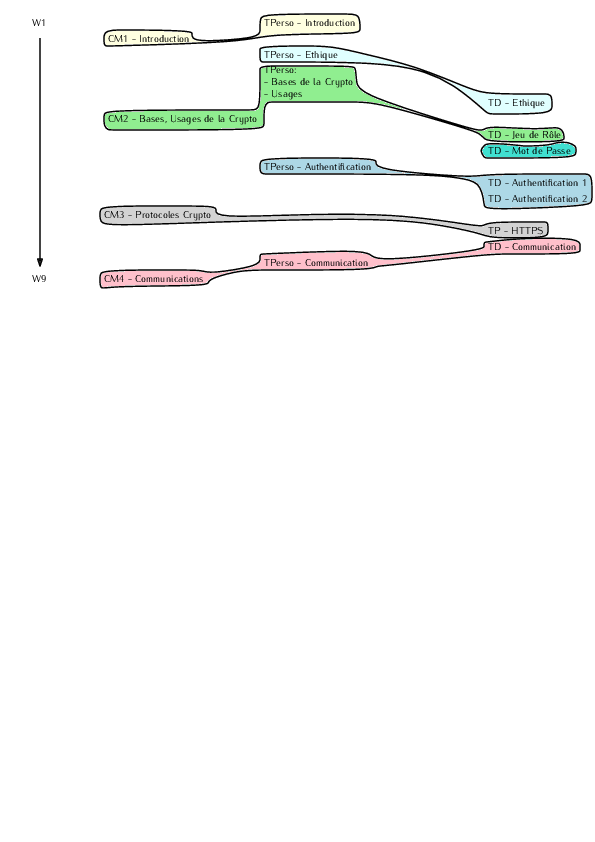
\includegraphics[width=\textwidth,keepaspectratio]{fig/CoursePlan.pdf}
  \end{center}  
\end{frame}


\begin{frame}
  \frametitle{Information Security}

  \begin{itemize}
  \item \textbf{Information security} $\triangleq$ practice of
    protecting information by mitigating information
    risks\footnote{\url{https://en.wikipedia.org/wiki/Information_security}}
  \item Need to protect all elements dealing with information: computers, networks, people
  \item Security covers a lot of different aspects:  physical security, social engineering, communication security, etc. 
  \item $\triangleq$ practice that allows to maintain the CIA triad (see next)
  \end{itemize}
\end{frame}


\begin{frame}
  \frametitle{The CIA Triad}
  \begin{itemize}
  \item \textbf{Confidentiality}: Information is not made available or
    disclosed to unauthorized individuals, entities, or
    processes.\footnote{Beckers, K. (2015). Pattern and Security
      Requirements: Engineering-Based Establishment of Security
      Standards.}
  \item \textbf{Integrity}: Information is not modified in an unauthorized or
    undetected manner. Also called \textbf{anti-tampering}.
  \item \textbf{Availability}: Information is available when it is needed.
  \end{itemize}
\end{frame}


\begin{frame}
  \frametitle{Threats}
  \begin{itemize}
  \item A \textbf{threat} is a potential negative action or event that can
    result in unwanted impact to a computer system, application or
    user information.
  \item A \textbf{threat model} is a set of properties that characterize
    threats associated to a particular environment. Often implies
    \textbf{security requirements} on a system. 
  \end{itemize}
\end{frame}


\begin{frame}
  \frametitle{Vulnerabilities}
  \begin{itemize}
  \item A \textbf{vulnerability} is a weakness which can be exploited by an
    attacker to access unauthorized information or to compromise the
    attacked system's behavior. 
  \item The \textbf{attack surface} of a system/application is the set of
    (known) vulnerabilities exposed by it to a potential attacker.
  \end{itemize}
\end{frame}


\begin{frame}
  \frametitle{Attacks}
  \begin{itemize}
  \item \textbf{Attack} = Attempt to exploit a vulnerability
  \item Attack can be:
    \begin{itemize}
    \item Passive (eavesdropping, side-channel, etc)
    \item Active (worm, faults, etc)
    \item Denial-of-service
    \end{itemize}
  \item When the attack is successful, we say the system is \textbf{compromised} 
  \end{itemize}
\end{frame}


\begin{frame}
  \frametitle{Trust}
  \begin{itemize}
  \item \textbf{Trust} = Degree to which an entity (person, system, hardware, software) is going to behave as expected
  \item A \textbf{Trust model} describes which entity(ies) is/are
    trusted and at which level.
  \end{itemize}
\end{frame}

\begin{frame}
  \frametitle{Threats and attack techniques - Examples}

  \begin{itemize}
  \item Eavesdropping, Trojans, Worms, Viruses
  \item Buffer Overflows, Spoofing, MITM attacks, Replay attacks, 
  \item Shoulder surfing, Dumpster diving, 
  \item Password attacks (brute-force, dictionary based), malicious-code attacks, 
  \item Side-channel attacks: cache, timing, power-monitoring, etc.
  \end{itemize}
\end{frame}



\begin{frame}
  \frametitle{}
  Quelques définitions:
  \begin{itemize}
  \item Trojan
  \item Worm
  \item Virus
  \item Buffer Overflow
  \item Spoofing
  \item Man-in-the-Middle Attack
  \item Replay
  \end{itemize}


  NB: donner 2 lignes pour chaque mot-clé. 
  
\end{frame}

\begin{frame}
  \frametitle{Defenses - a quick panorama}
  \begin{itemize}
  \item Cryptography
  \item Secured communication protocols
  \item Code and Data Encryption
  \item Physical shielding
  \item White-box cryptography    
  \end{itemize}
\end{frame}


\begin{frame}[fragile]
  \frametitle{Definition - Communication Security}

  \begin{block}{}
    \begin{center}
      \includegraphics[scale=1]{commSecurity.pdf}
    \end{center}
    \footnote{inspiration: \url{https://en.wikipedia.org/wiki/Communications_security}}
  \end{block}
\end{frame}


\begin{frame}
  \frametitle{Cryptology}

  Cryptology, is the science of practice and study of techniques for secure communication in the presence of adversarial behavior.

  \begin{itemize}
  \item \textbf{Cryptography}: Practice and study of techniques for secure communication in the presence of adversarial behavior.
  \item \textbf{Cryptanalysis}: Process of analyzing information systems in order to understand hidden aspects of the systems. 
  \item \textbf{Cryptology = Cryptography + Cryptanalysis}
  \end{itemize}

  In this course, we mainly focus on \textbf{Cryptography}. 
\end{frame}


\begin{frame}
  \frametitle{A brief history of cryptography}

  \begin{itemize}
  \item Keeping message secret has always been a (powerful) men's
    concern ...
  \item  ... but (at least today) it's also of every person's interest. 
  \item ... because there is no ``I got nothing to hide'' 
  \end{itemize}
\end{frame}


\begin{frame}
  \frametitle{A rajouter dans l'historique}

  Je repique du cours de François:
  \begin{itemize}
  \item La scytale
  \item Vigenère (mais j'ai pas encore compris)
  \item Vername (idem)
  \item Principe de Kerchoffs
  \item Confusion/Diffusion (Shannon 1949)
  \end{itemize}
  
\end{frame}


\begin{frame}
  \frametitle{History (1) Caesar cipher}

  \begin{itemize}
  \item Substitution cipher
  \item Each letter is encoded with its order in the alphabet: A$\rightarrow$0, B$\rightarrow$1, ..., Z$\rightarrow$26
  \item We choose a \textbf{fixed \textit{shift value}} $sh$
  \item To \textbf{encrypt}, each letter $P_i$ in Plaintext is replaced by the corresponding shifted letter:
    \begin{itemize}
    \item[] $\bm{E(P_i) = (P_i + sh) \mbox{ mod } 26}$
    \end{itemize}
  \item To \textbf{decrypt}, each letter $C_i$ in the Ciphertext is converted back with :
    \begin{itemize}
    \item[] $\bm{D(C_i) = (C_i - sh) \mbox{ mod } 26}$ 
    \end{itemize}
  \end{itemize}

  \putat{0.5}{0.75}{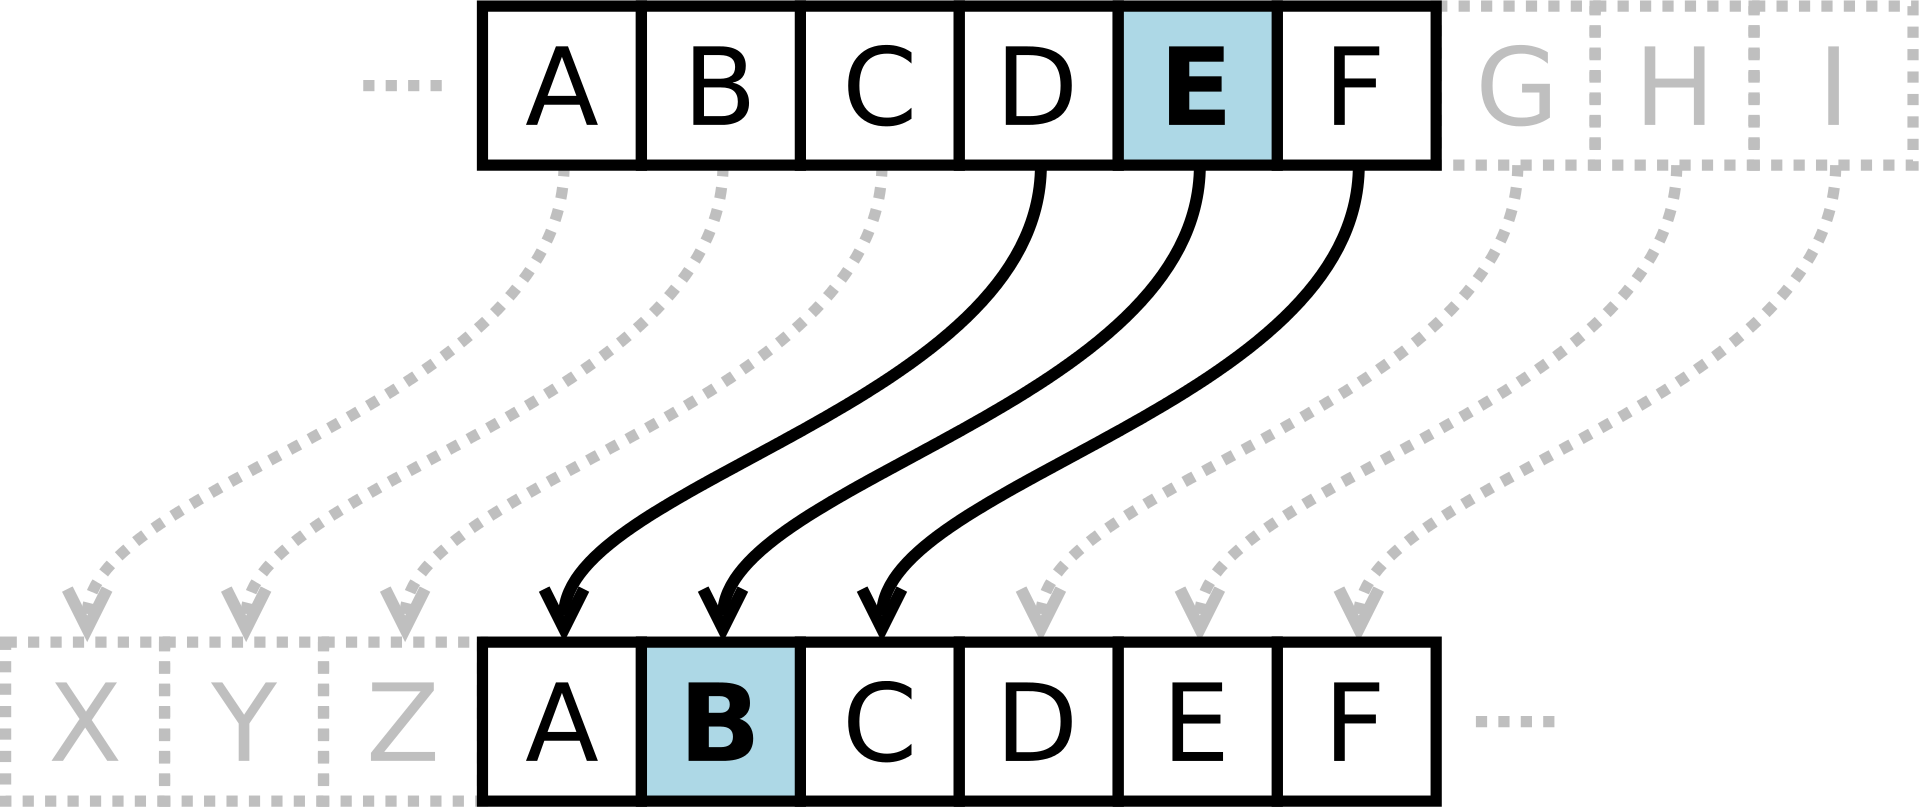
\includegraphics[scale=0.07]{Caesar_cipher_left_shift_of_3.png}}
  
\end{frame}



\begin{frame}
  \frametitle{History (1) Caesar cipher}
  \putat{0.4}{0.7}{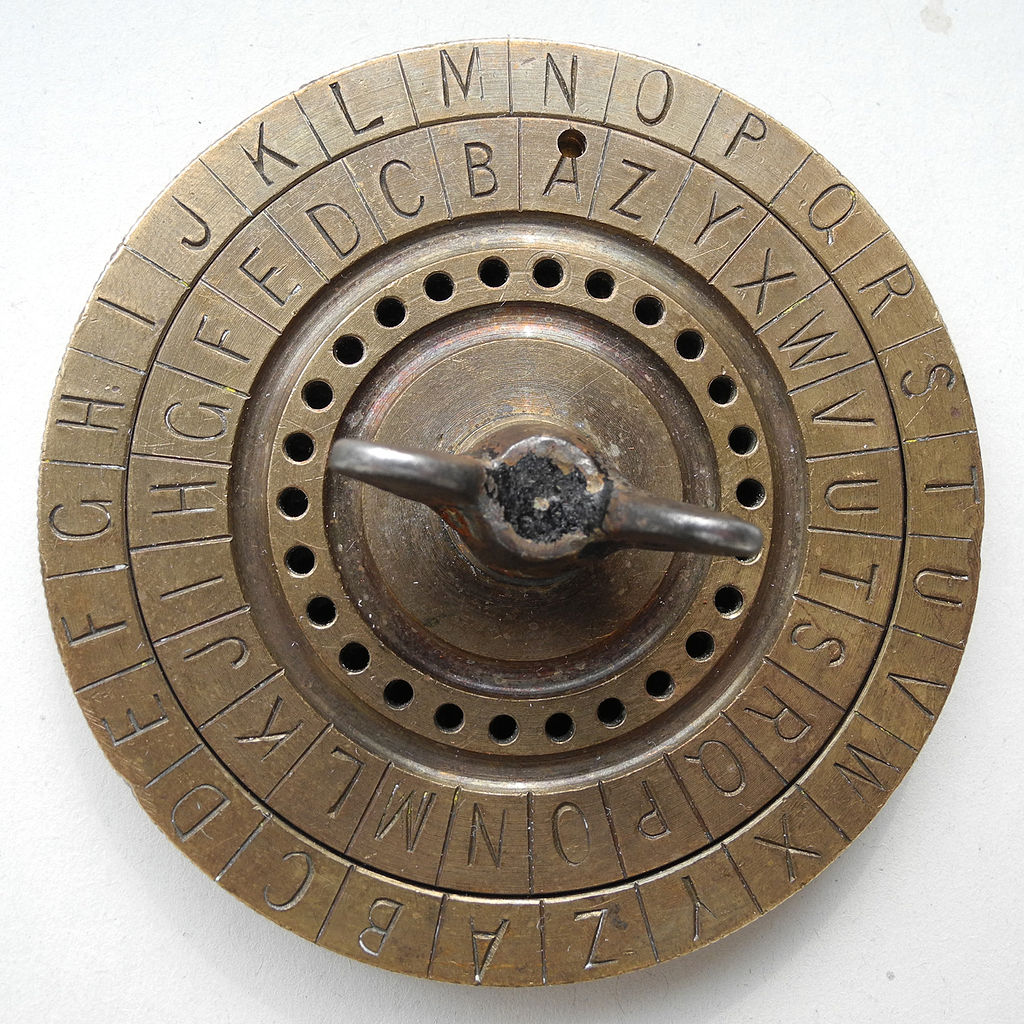
\includegraphics[scale=0.3]{1024px-CipherDisk2000.jpg}}
 
  \begin{itemize}
  \item[\plus] Encryption and decryption are cheap
  \item[\minus] Easy to crack with frequency analysis
  \item[\minus] Sufficient when no-one around can read :) (in
    particular, what's the difference between a foreign language and
    an encrypted language, if you can't read the first).
  \end{itemize}
\end{frame}


\begin{frame}
  \frametitle{One-time pad}
  \begin{itemize}
  \item Substitution cipher
  \item Choose a \textbf{random key $K$} as least as long as the plaintext
  \item To \textbf{encrypt}, each letter $P_i$ in Plaintext is replaced by the corresponding shifted letter:
    \begin{itemize}
    \item[] $\bm{E(P_i) = (P_i + K_i) \mbox{ mod } 26}$
    \end{itemize}
  \item To \textbf{decrypt}, each letter $C_i$ in the Ciphertext is converted back with :
    \begin{itemize}
    \item[] $\bm{D(C_i) = (C_i - K_i) \mbox{ mod } 26}$ 
    \end{itemize} 
  \end{itemize}
  \putat{0.7}{0.6}{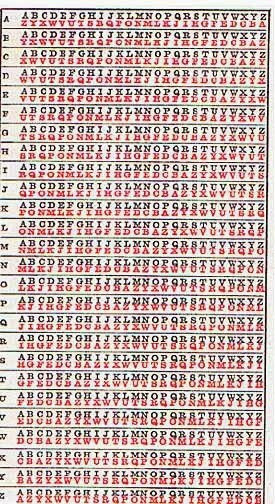
\includegraphics[scale=0.3]{onetimepad.jpg}}
  
\end{frame}


\begin{frame}
  \frametitle{One-time pad - Pros and Cons}

  \begin{itemize}
  \item[\plus] Proven secure
  \item[\plus] Even to frequency analysis
  \item[\plus] Encryption and decryption are cheap
  \item[\minus] Key must be as long as the plaintext ... 
  \item[\minus] Key must be kept secret
  \item[\minus] Key must not be lost (not by one character)  
  \item[\minus] Key must be truly random 
  \end{itemize}
\end{frame}

  
% \begin{frame}  
%   Un panorama de l'histoire de la sécurité des communications:
%   \begin{itemize}
%   \item Le code de César
%   \item ...
%   \item Le ``one-pad pads'' cipher (dont le problème résiduel considérable est que ça nécessite une clé
%     \begin{itemize}
%     \item Besoin de ``true randomness''
%     \item Peut-être je peux passer du temps à expliquer qu'obtenir du vrai random dans un ordinateur c'set dur. 
%     \item \url{https://www.youtube.com/watch?v=M8Tf9_O7s9c}
%     \end{itemize}
%   \item Enigma et la cryptanalyse de Turing et al
%   \end{itemize}
% \end{frame}


\begin{frame}
  \frametitle{Enigma}
  \putat{0.7}{0.6}{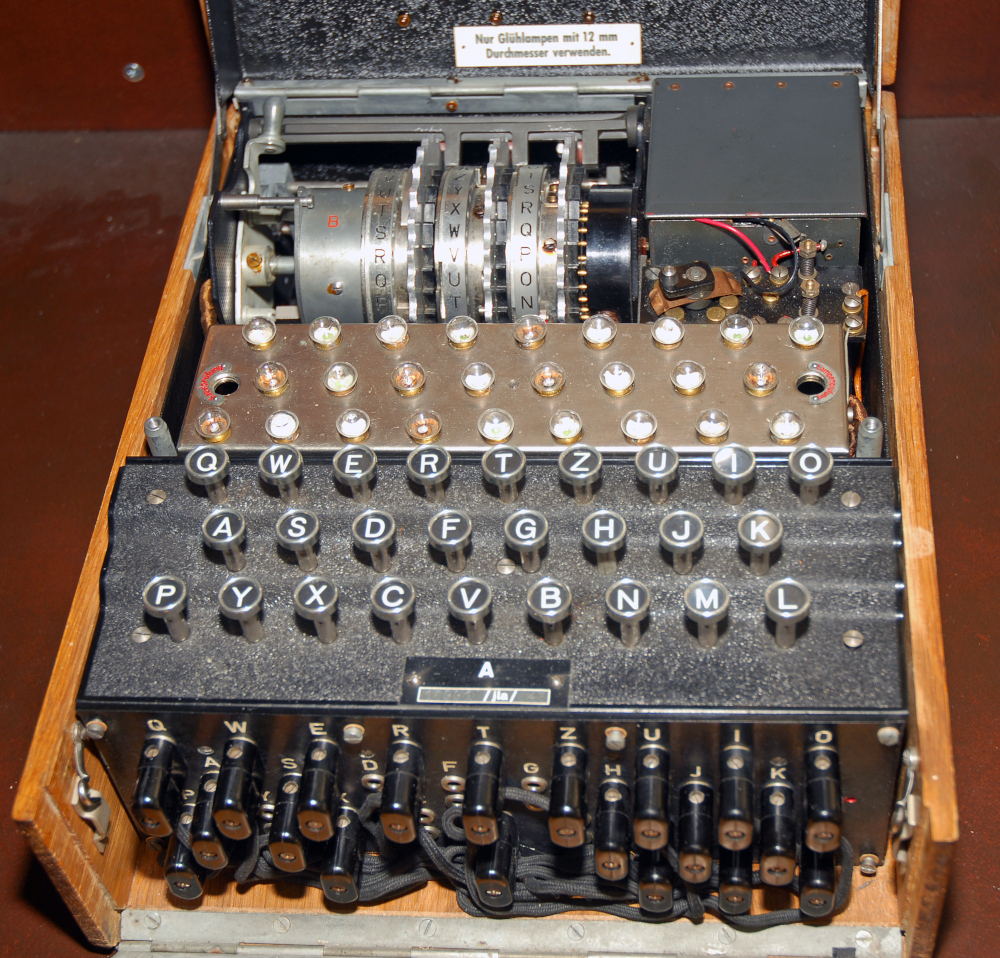
\includegraphics[scale=0.3]{enigma.jpg}}

  \begin{itemize}
  \item Invented at the end of WWI
  \item Used extensively by Nazi Germany during WWII
  \item First cracked by Polish services during the early 30s ... 
  \item ... then by British-led effort at Bletchley Park, including Alan Turing. 
  \end{itemize}
\end{frame}


\begin{frame}
  \frametitle{Enigma - How does it work?}

  \begin{itemize}
  \item Substitution cipher
  \end{itemize}

  \begin{center}
    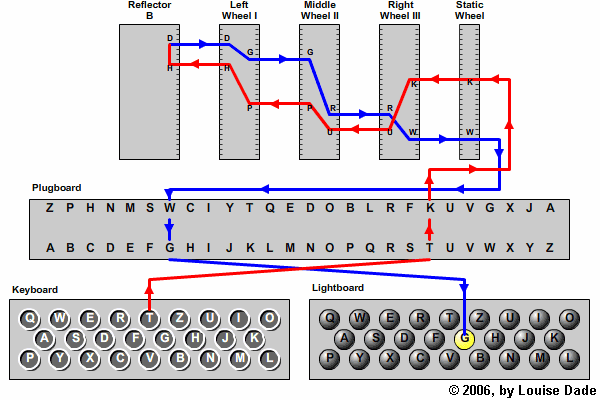
\includegraphics[scale=0.3]{Enigma-wiringdiagram.png}
  \end{center}
 
\end{frame}


\begin{frame}
  \frametitle{Enigma - Combinatorial}
  \begin{itemize}
  \item \textbf{Every day}, the machine is reset to a pre-established configuration:
    \begin{itemize}
    \item $20$ Rotors choice (3 or 4 or 5 among 6 possible). 
    \item $26^3$ Rotors permutation 
    \item  $26^3$Rotors initial positions 
    \item Plug-board settings: $150.10^{12}$
    \end{itemize}
  \item \textbf{Every message} contains a rotors position the machine
    should be reset to before decrypting the rest of the message.
  \end{itemize}  
\end{frame}

\begin{frame}
  \frametitle{Enigma - Breaking the machine}

  \begin{itemize}
  \item To brute-force Enigma is unpractical: 150 millions millions combinations
  \item A letter is encrypted into a different letter every time ....
  \item ... but never to itself !! \textbf{Main flaw}
  \item Try to guess a word or phrase in a message (and Germans military did use recurring messages, like weather reports)
  \item ... 
  \end{itemize}

\end{frame}

\begin{frame} 
  \frametitle{Enigma - breaking the machine}
  \begin{center}
    \only<1>{\includegraphics[scale=0.7,page=1]{exampleEnigma.pdf}}
    \only<2>{\includegraphics[scale=0.7,page=2]{exampleEnigma.pdf}}
    \only<3>{\includegraphics[scale=0.7,page=3]{exampleEnigma.pdf}}
    \only<4>{\includegraphics[scale=0.7,page=4]{exampleEnigma.pdf}}
    \only<5>{\includegraphics[scale=0.7,page=5]{exampleEnigma.pdf}}
  \end{center}
\end{frame}

\begin{frame}[fragile]
  \frametitle{Enigma - Breaking the machine}

  \begin{itemize}
  \item Adding a couple more properties, evict impossible configurations. 
  \item Scan through the remaining combinations using \textbf{the Bombe} : electro-mechanical machine able to ``play'' 36 Enigma equivalent ``in parallel''. 
  \item In the end .... guess the key (wheel starting positions + plug-board) in less than 20minutes per day. 
  \end{itemize}
 
\end{frame}



\begin{frame}
    \frametitle{Enigma}
  \begin{minipage}{0.45\textwidth}
    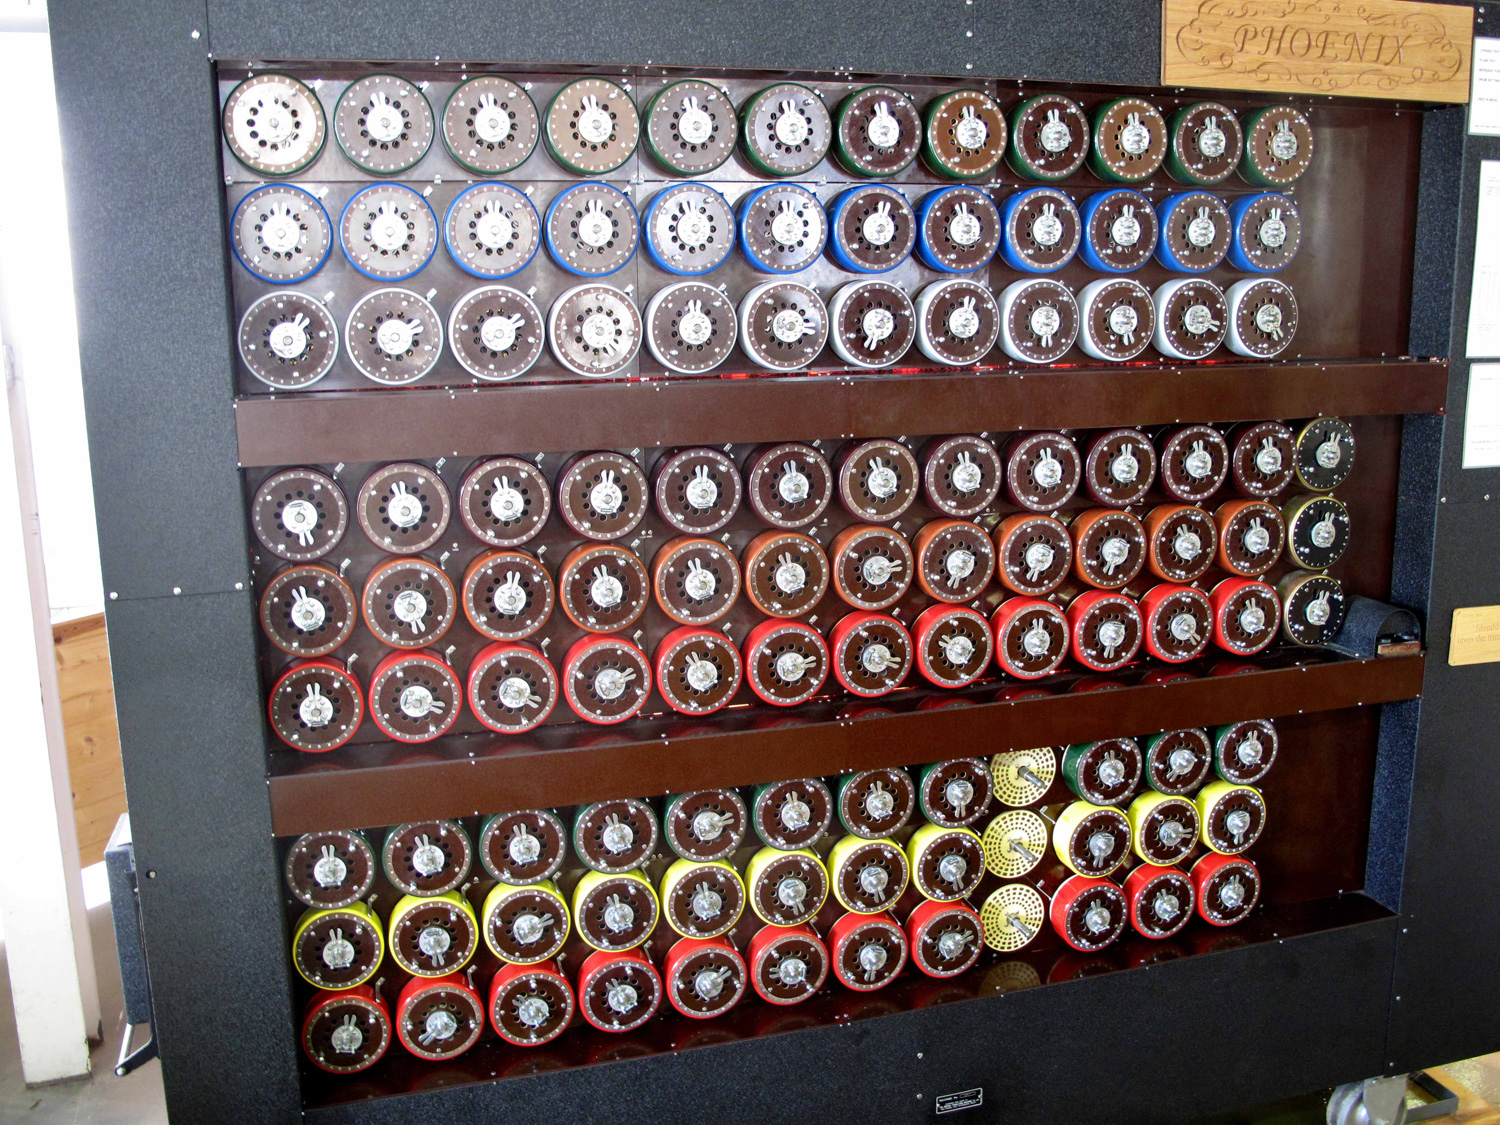
\includegraphics[scale=0.1]{rebuilt-bombe-bletchley-park.jpg}
  \end{minipage}
  \hfill
  \begin{minipage}{0.45\textwidth}
    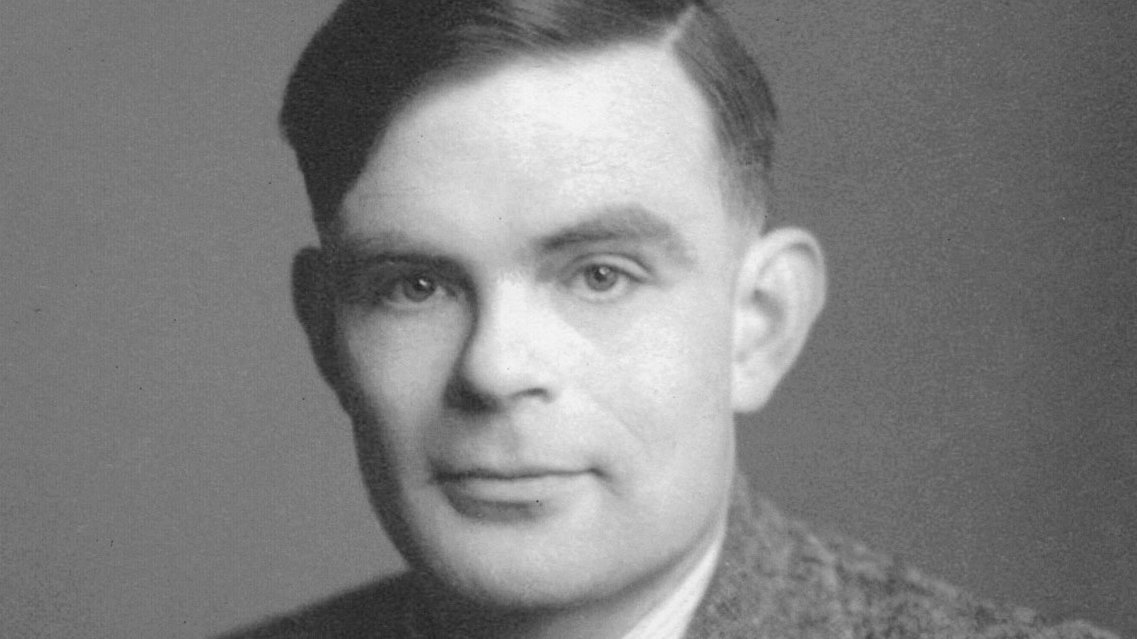
\includegraphics[scale=0.1]{alanTuring.jpg}
  \end{minipage}

  \footnote*{watch \url{https://en.wikipedia.org/wiki/The_Imitation_Game}}
  
\end{frame}


\begin{frame}
  \frametitle{Next time - Cryptography}
  \begin{itemize}
  \item Symmetric cryptography
  \item Asymmetric cryptography
  \item Key sharing
  \end{itemize}
  
\end{frame}

\end{document}

  